% !TEX program = xelatex
\documentclass[a4paper,10pt]{article}

\makeatletter
\let\@expl@@@mark@update@singlecol@structures@@\relax
\makeatother

\usepackage[a4paper, left=1.0cm, right=1.0cm, top=0.90cm, bottom=1.05cm, footskip=0.48cm]{geometry}
\usepackage{fontspec}
\usepackage{amsmath, amssymb}
\usepackage{array, colortbl}
\usepackage[table]{xcolor}
\usepackage{tcolorbox}
\tcbuselibrary{skins, breakable}
\usepackage{fancyhdr}
\usepackage{enumitem}
\usepackage{tikz}
\usetikzlibrary{calc, angles, quotes, arrows.meta}

\makeatletter
\newcommand{\NGSFindFonts}{%
  \IfFileExists{../../../fonts/KhmerOSsiemreap.ttf}{%
    \def\NGSUserPath{../../../fonts/}\def\NGSSysPath{../../../fonts/}%
  }{%
    \IfFileExists{../../../../fonts/KhmerOSsiemreap.ttf}{%
      \def\NGSUserPath{../../../../fonts/}\def\NGSSysPath{../../../../fonts/}%
    }{%
      \IfFileExists{fonts/KhmerOSsiemreap.ttf}{%
        \def\NGSUserPath{fonts/}\def\NGSSysPath{fonts/}%
      }{%
        \def\NGSUserPath{C:/Users/user/AppData/Local/Microsoft/Windows/Fonts/}%
        \def\NGSSysPath{C:/Windows/Fonts/}%
      }%
    }%
  }%
}
\NGSFindFonts
\makeatother

\XeTeXlinebreaklocale "km"
\XeTeXlinebreakskip = 0pt plus 1pt minus 0.1pt

\setmainfont[
  Path = {\NGSUserPath},
  Extension = .ttf,
  UprightFont = KhmerOSsiemreap,
  BoldFont = KhmerOSsiemreap,
  BoldFeatures = {FakeBold=1.8},
  ItalicFont = KhmerOSsiemreap,
  ItalicFeatures = {FakeSlant=0.25}
]{KhmerOSsiemreap}

\newfontfamily\muol[Path={\NGSUserPath}]{KhmerOSmuollight.ttf}
\newfontfamily\enfont[Path={\NGSSysPath}, Scale=1.0]{times.ttf}
\newfontfamily\enbold[Path={\NGSSysPath}, Scale=1.0]{timesbd.ttf}
\newfontfamily\calibrifont[Path={\NGSSysPath}, Scale=0.95]{calibri.ttf}

\DeclareTextFontCommand{\en}{\enfont}
\newcommand{\enbf}[1]{{\enbold #1}}

\definecolor{headgray}{HTML}{E2E2E2}
\definecolor{panelgray}{HTML}{F5F5F5}

\pagestyle{fancy}
\fancyhf{}
\renewcommand{\headrulewidth}{0pt}
\renewcommand{\footrulewidth}{0.4pt}
\fancyfoot[L]{\rule{0pt}{11pt}\fontsize{8.5pt}{11pt}\selectfont អនុវិទ្យាល័យព្រះក្រសាំង $\;\vert\;$ គណិតវិទ្យា ថ្នាក់ទី៨ $\;\vert\;$ មេរៀនទី១៤ (១៤.៤) លំហាត់សំយោគផ្ទៃក្រឡាពហុកោណ}
\fancyfoot[R]{\rule{0pt}{11pt}\fontsize{8.5pt}{11pt}\selectfont ទំព័រ \en{\thepage\,/\,2}}

\setlength{\parindent}{0pt}
\setlength{\tabcolsep}{4pt}

\newcommand{\tri}[1]{\triangle #1}
\newcommand{\unit}[1]{\,\text{\en{#1}}}
\newcommand{\blank}[1]{\leavevmode\hbox to #1{\dotfill}}
\newcommand{\chkbox}{\tikz[baseline=0.2ex]\draw[black, line width=0.7pt] (0,0) rectangle (1.55ex,1.55ex);}
\newcommand{\cnum}[1]{\tikz[baseline=-0.58ex]\node[circle, fill=black, text=white, inner sep=0.85pt, minimum size=1.95ex, font=\enbold\scriptsize]{#1};}

\newcommand{\rightbox}[4][0.20cm]{%
  \coordinate (rbA) at ($(#3)!#1!(#2)$);
  \coordinate (rbB) at ($(#3)!#1!(#4)$);
  \coordinate (rbC) at ($(rbA)+(#3)!#1!(#4)-(#3)$);
  \draw[black, line width=0.65pt] (rbA) -- (rbC) -- (rbB);
}

\newcommand{\secbar}[2]{%
  \vspace{2.5pt}%
  \begin{tcolorbox}[
    enhanced, sharp corners, colback=headgray, colframe=black,
    boxrule=0.85pt, left=6pt, right=6pt, top=2.5pt, bottom=2.5pt, after skip=3.5pt
  ]
    {\muol\fontsize{9.5pt}{14pt}\selectfont #1}\hfill{\fontsize{9pt}{13pt}\selectfont\textbf{#2}}
  \end{tcolorbox}%
}

\begin{document}
\fontsize{9.6pt}{14.2pt}\selectfont

% ==================== ក្បាលសន្លឹកកិច្ចការ ====================
\begin{tcolorbox}[
  enhanced, sharp corners, colback=white, colframe=black,
  boxrule=1.1pt, left=6pt, right=6pt, top=3.5pt, bottom=3.5pt, after skip=3pt
]
  \begin{minipage}[c]{11.5cm}
    {\muol\fontsize{10.5pt}{15.5pt}\selectfont សន្លឹកកិច្ចការសិស្ស — មេរៀនទី១៤ ៖ ផ្ទៃក្រឡាពហុកោណ}\\[1.5pt]
    \textbf{ចំណុចទី ៤ ៖ លំហាត់អនុវត្ត និងចំណោទសំយោគ} (សៀវភៅសិក្សាគោល ទំ.១៩៤--១៩៦)
  \end{minipage}\hfill
  \begin{minipage}[c]{6.9cm}
    ឈ្មោះសិស្ស៖ \blank{4.6cm}\\[2pt]
    ថ្នាក់ទី៨៖ \blank{1.4cm} \hspace{0.2cm} ដៃគូទី៖ \blank{2.1cm}
  \end{minipage}
\end{tcolorbox}

% ==================== ផ្នែកទី ១ ៖ E1 - ENGAGE ====================
\secbar{ផ្នែកទី ១ ៖ បេសកកម្មវិស្វកម្ម (\enbf{E1}) — ផ្ទាំងកញ្ចក់ជ្រុងអគារធំ (លំហាត់ទី១០ ទំ.១៩៦)}{\en{3} នាទី (ទស្សន៍ទាយមុនរៀន)}

\begin{tcolorbox}[
  enhanced, sharp corners, colback=panelgray, colframe=black,
  boxrule=0.8pt, left=6pt, right=6pt, top=3pt, bottom=3pt, after skip=3pt
]
  \begin{minipage}[c]{12.0cm}
    ជ្រុងម្ខាងនៃអគារទំនើបមួយមានរាងជា \textbf{ចតុកោណព្នាយ} ដែលបាតក្រោមមានប្រវែង $b = 400\unit{m}$, ដំបូលខាងលើមានប្រវែង $b' = 150\unit{m}$ និងកម្ពស់អគារមានប្រវែង $h = 500\unit{m}$។ បើគេបំពាក់ផ្ទាំងកញ្ចក់ពេញជ្រុងអគារនេះ ដោយកញ្ចក់ ១ ផ្ទាំងមានផ្ទៃ $1\unit{m}^2$ តើគេត្រូវប្រើកញ្ចក់អស់ប៉ុន្មានផ្ទាំង?\\[2pt]
    \textbf{ការប៉ាន់ស្មានដំបូង៖} \hspace{0.15cm}
    \chkbox\ $75\,000$ ផ្ទាំង \hspace{0.35cm}
    \chkbox\ $137\,500$ ផ្ទាំង \hspace{0.35cm}
    \chkbox\ $275\,000$ ផ្ទាំង \hspace{0.35cm}
    \chkbox\ មិនទាន់ប្រាកដ
  \end{minipage}\hfill
  \begin{minipage}[c]{6.2cm}
    \centering
    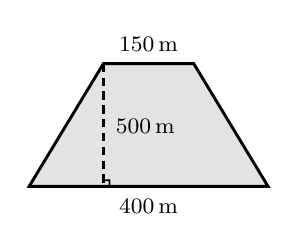
\begin{tikzpicture}[scale=0.41, every node/.style={font=\footnotesize, text=black}]
      \coordinate (D) at (0,0);
      \coordinate (C) at (7.4,0);
      \coordinate (B) at (5.1,3.8);
      \coordinate (A) at (2.3,3.8);
      \coordinate (H) at (2.3,0);
      \fill[gray!22] (D)--(C)--(B)--(A)--cycle;
      \draw[black, line width=1.05pt] (D)--(C)--(B)--(A)--cycle;
      \draw[black, line width=0.85pt, densely dashed] (A)--(H);
      \rightbox[0.19cm]{A}{H}{C}
      \node[above=1pt] at (3.7,3.8) {$150\unit{m}$};
      \node[below=1pt] at (3.7,0) {$400\unit{m}$};
      \node[right=1pt] at (2.3,1.85) {$500\unit{m}$};
    \end{tikzpicture}
  \end{minipage}
\end{tcolorbox}

% ==================== ផ្នែកទី ២ ៖ E2 - EXPLORE ====================
\secbar{ផ្នែកទី ២ ៖ យុទ្ធវិធីស៊ុមដកផ្នែកស សម្រាប់ពហុកោណប្រផេះទ្រេត និងផត (\enbf{E2 — Explore})}{\en{11} នាទី (ពិភាក្សាដៃគូ)}

\begin{minipage}[c]{6.8cm}
  \centering
  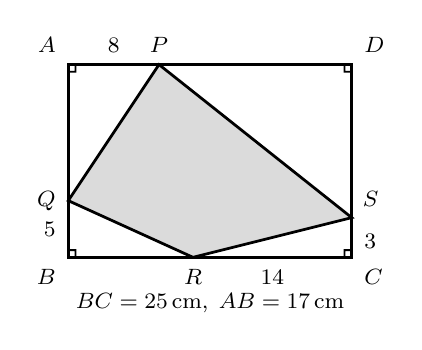
\begin{tikzpicture}[scale=0.48, every node/.style={font=\footnotesize, text=black}]
    \coordinate (B) at (0,0);
    \coordinate (C) at (7.5,0);
    \coordinate (D) at (7.5,5.1);
    \coordinate (A) at (0,5.1);
    \coordinate (P) at (2.4,5.1);
    \coordinate (Q) at (0,1.5);
    \coordinate (R) at (3.3,0);
    \coordinate (S) at (7.5,1.05);
    \fill[gray!28] (P)--(Q)--(R)--(S)--cycle;
    \draw[black, line width=1.05pt] (A)--(B)--(C)--(D)--cycle;
    \draw[black, line width=1.0pt] (P)--(Q)--(R)--(S)--cycle;
    \rightbox[0.19cm]{P}{A}{Q}\rightbox[0.19cm]{Q}{B}{R}
    \rightbox[0.19cm]{R}{C}{S}\rightbox[0.19cm]{S}{D}{P}
    \node[above left=1pt] at (A) {$A$};
    \node[below left=1pt] at (B) {$B$};
    \node[below right=1pt] at (C) {$C$};
    \node[above right=1pt] at (D) {$D$};
    \node[above=1pt] at (P) {$P$};
    \node[left=1pt] at (Q) {$Q$};
    \node[below=1pt] at (R) {$R$};
    \node[above right=0.5pt] at (S) {$S$};
    \node[above=1pt] at (1.2,5.1) {$8$};
    \node[left=1pt] at (0,0.75) {$5$};
    \node[below=1pt] at (5.4,0) {$14$};
    \node[right=1pt] at (7.5,0.42) {$3$};
    \node[below=2pt] at (3.75,-0.55) {$BC = 25\unit{cm},\; AB = 17\unit{cm}$};
  \end{tikzpicture}
\end{minipage}\hfill
\begin{minipage}[c]{11.7cm}
  \textbf{(ក) លំហាត់ទី ៥ (ទំ.១៩៤)៖} ចតុកោណកែង $ABCD$ មាន $AB = 17\unit{cm},\; BC = 25\unit{cm}$ ហើយ $AP = 8\unit{cm},\; BQ = 5\unit{cm},\; CR = 14\unit{cm},\; CS = 3\unit{cm}$។
  \begin{enumerate}[label=\enbf{\arabic*.}, leftmargin=1.4em, itemsep=2pt, topsep=1.5pt]
    \item រកប្រវែងជ្រុងនៅសល់តាមកែងទាំង ៤៖\\
    $AQ = 17 - 5 =$ \blank{1.0cm} $\;\vert\;$ $BR = 25 - 14 =$ \blank{1.0cm}\\
    $PD = 25 - 8 =$ \blank{1.0cm} $\;\vert\;$ $DS = 17 - 3 =$ \blank{1.0cm}
    \item គណនាផ្ទៃស៊ុមធំ៖ $S_{ABCD} = 17 \times 25 =$ \blank{1.6cm} $\unit{cm}^2$។
    \item គណនាផ្ទៃត្រីកោណកែងពណ៌សទាំង ៤ ជ្រុង៖\\
    $S_{\tri{APQ}} = \frac{1}{2}(8)(12) =$ \blank{1.1cm} $\;\vert\;$ $S_{\tri{BQR}} = \frac{1}{2}(5)(11) =$ \blank{1.2cm}\\
    $S_{\tri{CRS}} = \frac{1}{2}(14)(3) =$ \blank{1.1cm} $\;\vert\;$ $S_{\tri{DPS}} = \frac{1}{2}(17)(14) =$ \blank{1.2cm}
    \item ដកផ្ទៃសសរុបចេញពីផ្ទៃស៊ុម៖ $S_{PQRS} = 425 - ($ \blank{1.6cm} $) =$ \blank{1.6cm} $\unit{cm}^2$។
  \end{enumerate}
\end{minipage}

\vspace{3pt}
\begin{tcolorbox}[
  enhanced, sharp corners, colback=panelgray, colframe=black,
  boxrule=0.8pt, left=6pt, right=6pt, top=3pt, bottom=3pt, after skip=3pt
]
  \begin{minipage}[c]{13.2cm}
    \textbf{(ខ) លំហាត់ទី ៦ រូបទី៣ (ទំ.១៩៥ — រូបព្រួញផត)៖} រូបព្រួញប្រផេះខាងស្ដាំកើតពីត្រីកោណធំ (បាត $19\unit{cm}$, កម្ពស់ $15\unit{cm}$) ដកត្រីកោណពណ៌សខាងក្រោម (បាតរួម $19\unit{cm}$, កម្ពស់ $7\unit{cm}$)៖\\[2pt]
    $S_{\text{ប្រផេះ}} = S_{\text{ធំ}} - S_{\text{ស}} = \dfrac{1}{2} \times 19 \times \blank{1.0cm} - \dfrac{1}{2} \times 19 \times \blank{1.0cm} =$ \blank{1.5cm} $-$ \blank{1.5cm} $=$ \blank{1.6cm} $\unit{cm}^2$។
  \end{minipage}\hfill
  \begin{minipage}[c]{5.0cm}
    \centering
    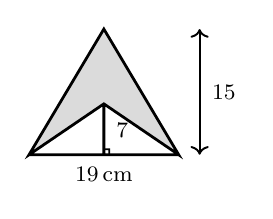
\begin{tikzpicture}[scale=0.38, every node/.style={font=\footnotesize, text=black}]
      \coordinate (L) at (0,0); \coordinate (R2) at (5.0,0);
      \coordinate (T) at (2.5,4.2); \coordinate (M) at (2.5,1.7); \coordinate (H) at (2.5,0);
      \fill[gray!28] (L)--(T)--(R2)--(M)--cycle;
      \draw[black, line width=1.0pt] (L)--(T)--(R2)--(M)--cycle (L)--(R2) (M)--(H);
      \draw[black, line width=0.7pt, <->] (5.7,0)--(5.7,4.2);
      \rightbox[0.18cm]{M}{H}{R2}
      \node[right=1pt] at (5.7,2.1) {$15$};
      \node[right=1pt] at (2.5,0.8) {$7$};
      \node[below=1pt] at (2.5,0) {$19\unit{cm}$};
    \end{tikzpicture}
  \end{minipage}
\end{tcolorbox}

% ==================== ផ្នែកទី ៣ ៖ E3 - EXPLAIN ====================
\secbar{ផ្នែកទី ៣ ៖ តារាងសំយោគរូបមន្តពហុកោណទាំង ៤ និងក្បួនយុទ្ធវិធី (\enbf{E3 — Explain})}{\en{6} នាទី}

\begin{tcolorbox}[
  enhanced, sharp corners, colback=white, colframe=black,
  boxrule=1.0pt, boxsep=2pt, top=3.5pt, bottom=3.5pt, left=6pt, right=6pt, after skip=3.5pt
]
  \renewcommand{\arraystretch}{1.16}
  \begin{tabular}{|p{4.3cm}|p{4.0cm}|p{4.4cm}|p{4.5cm}|}
    \hline
    \cellcolor{headgray}\centering\textbf{១. ប្រលេឡូក្រាម} &
    \cellcolor{headgray}\centering\textbf{២. ត្រីកោណ} &
    \cellcolor{headgray}\centering\textbf{៣. ចតុកោណស្មើ} &
    \cellcolor{headgray}\centering\arraybackslash\textbf{៤. ចតុកោណព្នាយ} \\[2pt]
    \hline
    \centering $S = b \times h$ \par ($h \perp b$) &
    \centering $S = \dfrac{1}{2} b \times h$ \par ($h$ ក្នុង ឬក្រៅ) &
    \centering $S = \dfrac{1}{2} d \times d'$ \par ($d, d'$ អង្កត់ទ្រូងពេញ) &
    \centering\arraybackslash $S = \dfrac{(b + b') \times h}{2}$ \par ($b \parallel b',\; h \perp b$) \\[2pt]
    \hline
    \centering រក $h = \dfrac{S}{\blank{0.8cm}}$ &
    \centering រក $h = \dfrac{2S}{\blank{0.8cm}}$ &
    \centering រក $d' = \dfrac{2S}{\blank{0.8cm}}$ &
    \centering\arraybackslash រក $h = \dfrac{2S}{\blank{1.3cm}}$ \\[4pt]
    \hline
  \end{tabular}\\[3.5pt]
  $\bullet$ \textbf{ក្បួនយុទ្ធវិធី៖} \cnum{1} \textbf{ពុះបូក៖} $S = S_1 + S_2$ $\;\vert\;$ \cnum{2} \textbf{ស៊ុមដកផ្នែកស៖} $S = S_{\text{ស៊ុម}} - S_{\text{ស}}$ $\;\vert\;$ \cnum{3} \textbf{ខ្នាតដី៖} $1\unit{ha} = 10\,000\unit{m}^2,\; 1\unit{km}^2 = 100\unit{ha}$។
\end{tcolorbox}

% បន្ថែមលំហាត់ប្រៀបធៀបវិធីពុះបូក (លំហាត់ទី ៧ រូបទី១ ទំ.១៩៦) ដើម្បីប្រើក្រដាសទំព័រទី១ ឱ្យអស់លទ្ធភាព
\begin{tcolorbox}[
  enhanced, sharp corners, colback=panelgray, colframe=black,
  boxrule=0.85pt, left=6pt, right=6pt, top=3pt, bottom=3pt
]
  \begin{minipage}[c]{13.3cm}
    \textbf{ផ្ទៀងផ្ទាត់ការជ្រើសរើសយុទ្ធវិធី (លំហាត់ទី ៧ រូបទី១ ទំ.១៩៦ — រូបមុខផ្ទះ)៖}\\
    រូបមុខផ្ទះខាងស្ដាំផ្គុំពីចតុកោណកែង ($10 \times 6$) បន្តុបត្រីកោណដំបូល (បាត $10$, កម្ពស់ $4$)។\\[2pt]
    ១. តើគួរជ្រើសរើសយុទ្ធវិធីណា? \hspace{0.2cm} \chkbox\ \cnum{1} វិធីពុះបូក ($S_1 + S_2$) \hspace{0.35cm} \chkbox\ \cnum{2} វិធីស៊ុមដកផ្នែកស\\[2pt]
    ២. គណនាផ្ទៃសរុប៖ $S = (10 \times \blank{0.9cm}) + \left(\dfrac{1}{2} \times 10 \times \blank{0.9cm}\right) =$ \blank{1.2cm} $+$ \blank{1.2cm} $=$ \blank{1.4cm}។
  \end{minipage}\hfill
  \begin{minipage}[c]{4.9cm}
    \centering
    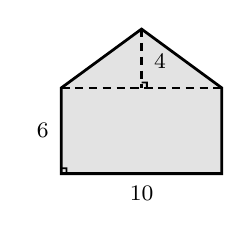
\begin{tikzpicture}[scale=0.34, every node/.style={font=\footnotesize, text=black}]
      \fill[gray!22] (0,0)--(6.0,0)--(6.0,3.2)--(3.0,5.4)--(0,3.2)--cycle;
      \draw[black, line width=1.0pt] (0,0)--(6.0,0)--(6.0,3.2)--(3.0,5.4)--(0,3.2)--cycle;
      \draw[black, line width=0.8pt, densely dashed] (0,3.2)--(6.0,3.2) (3.0,5.4)--(3.0,3.2);
      \rightbox[0.20cm]{0,3.2}{0,0}{6.0,0}\rightbox[0.20cm]{3.0,5.4}{3.0,3.2}{6.0,3.2}
      \node[below=1pt] at (3.0,0) {$10$};
      \node[left=1pt] at (0,1.6) {$6$};
      \node[right=1pt] at (3.0,4.2) {$4$};
    \end{tikzpicture}
  \end{minipage}
\end{tcolorbox}

\newpage

% ==================== ទំព័រទី ២ ៖ E4, E5 និងកិច្ចការផ្ទះ ====================
\secbar{ផ្នែកទី ៤ ៖ ចំណោទអនុវត្តជីវភាពពិតតាមជំហាន \enbf{Polya} (\enbf{E4 — Elaborate})}{\en{10} នាទី (ទំ.១៩៦)}

\begin{tcolorbox}[
  enhanced, sharp corners, colback=white, colframe=black,
  boxrule=0.95pt, boxsep=2pt, top=4pt, bottom=4pt, left=6pt, right=6pt, after skip=5pt
]
  \begin{minipage}[c]{12.4cm}
    \textbf{លំហាត់ទី ៨ (ទំ.១៩៦ — ចំការកៅស៊ូ និងការបម្លែងខ្នាតហិចតា)៖}\\
    ចំការកៅស៊ូមួយមានរាងជាចតុកោណកែងដែលមានបណ្ដោយប្រវែង $5\unit{km}$ និងទទឹងប្រវែង $2.3\unit{km}$។ គណនាផ្ទៃក្រឡាចំការកៅស៊ូគិតជា \textbf{ហិចតា ($\unit{ha}$)}។
    \begin{itemize}[leftmargin=1.2em, itemsep=2.5pt, topsep=2pt]
      \item \textbf{ជំហានទី ១ (សម្មតិកម្ម និងផ្ទៃគិតជា $\unit{km}^2$)៖} $b = 5\unit{km},\; h = 2.3\unit{km} \Rightarrow S = 5 \times 2.3 =$ \blank{1.6cm} $\unit{km}^2$។
      \item \textbf{ជំហានទី ២ (បម្លែងខ្នាតតាម \cnum{3} ៖ $1\unit{km}^2 = 100\unit{ha}$)៖} $S =$ \blank{1.5cm} $\times 100 =$ \blank{2.0cm} ហិចតា ($\unit{ha}$)។
      \item \textbf{ជំហានទី ៣ (ផ្ទៀងផ្ទាត់ និងឆ្លើយ)៖} ដូចនេះ ចំការកៅស៊ូមានផ្ទៃក្រឡាសរុប \blank{2.2cm} ហិចតា។
    \end{itemize}
  \end{minipage}\hfill
  \begin{minipage}[c]{5.6cm}
    \centering
    \begin{tikzpicture}[scale=0.46, every node/.style={font=\footnotesize, text=black}]
      \fill[gray!18] (0,0) rectangle (6.0,2.9);
      \draw[black, line width=1.05pt] (0,0) rectangle (6.0,2.9);
      \rightbox[0.19cm]{0,2.9}{0,0}{6.0,0}
      \node[below=1.5pt] at (3.0,0) {$5\unit{km}$};
      \node[left=1.5pt] at (0,1.45) {$2.3\unit{km}$};
      \node at (3.0,1.45) {ចំការកៅស៊ូ};
    \end{tikzpicture}
  \end{minipage}
\end{tcolorbox}

\begin{tcolorbox}[
  enhanced, sharp corners, colback=white, colframe=black,
  boxrule=0.95pt, boxsep=2pt, top=4pt, bottom=4pt, left=6pt, right=6pt, after skip=5pt
]
  \begin{minipage}[c]{12.4cm}
    \textbf{លំហាត់ទី ៩ (ទំ.១៩៦ — សួនច្បារផ្កាកុលាបរាងត្រីកោណ)៖}\\
    សួនច្បារផ្កាកុលាបមួយមានរាងជាត្រីកោណដែលមានបាត $5\unit{m}$ និងកម្ពស់ $3\unit{m}$។ បើគេដាំផ្កាកុលាបមួយដើមត្រូវការផ្ទៃដី $0.5\unit{m}^2$ តើគេអាចដាំផ្កាកុលាបបានប៉ុន្មានដើមក្នុងសួនច្បារនេះ?
    \begin{itemize}[leftmargin=1.2em, itemsep=2.5pt, topsep=2pt]
      \item \textbf{ជំហានទី ១ (ផ្ទៃសួនរាងត្រីកោណ)៖} $S = \dfrac{1}{2} \times \blank{1.0cm} \times \blank{1.0cm} =$ \blank{1.8cm} $\unit{m}^2$។
      \item \textbf{ជំហានទី ២ (ចំនួនដើមផ្កា៖ $N = S \div S_{\text{១ដើម}}$)៖} $N =$ \blank{1.4cm} $\div 0.5 =$ \blank{1.8cm} ដើម។
      \item \textbf{ជំហានទី ៣ (ផ្ទៀងផ្ទាត់៖ $N \times 0.5 = S$)៖} \blank{1.3cm} $\times 0.5 =$ \blank{1.4cm} $\unit{m}^2$ (ពិត)។
    \end{itemize}
  \end{minipage}\hfill
  \begin{minipage}[c]{5.6cm}
    \centering
    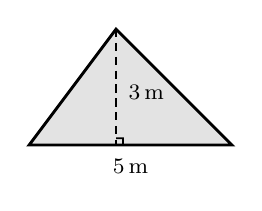
\begin{tikzpicture}[scale=0.46, every node/.style={font=\footnotesize, text=black}]
      \coordinate (A) at (0,0); \coordinate (B) at (5.6,0);
      \coordinate (C) at (2.4,3.2); \coordinate (H) at (2.4,0);
      \fill[gray!22] (A)--(B)--(C)--cycle;
      \draw[black, line width=1.05pt] (A)--(B)--(C)--cycle;
      \draw[black, line width=0.85pt, densely dashed] (C)--(H);
      \rightbox[0.19cm]{C}{H}{B}
      \node[below=1.5pt] at (2.8,0) {$5\unit{m}$};
      \node[right=1pt] at (2.4,1.45) {$3\unit{m}$};
    \end{tikzpicture}
  \end{minipage}
\end{tcolorbox}

% ==================== ផ្នែកទី ៥ ៖ E5 - EVALUATE ====================
\secbar{ផ្នែកទី ៥ ៖ លំហាត់វាយតម្លៃសំយោគ និងបិទបេសកកម្ម (\enbf{E5 — Evaluate})}{\en{10} នាទី (ទំ.១៩៥--១៩៦)}

\begin{minipage}[t]{9.2cm}
  \begin{tcolorbox}[
    enhanced, sharp corners, colback=white, colframe=black,
    boxrule=0.95pt, boxsep=2pt, top=4pt, bottom=4pt, left=5pt, right=5pt, equal height group=e5area4
  ]
    \textbf{ក. លំហាត់ទី ៦ រូបទី១ (ទំ.១៩៥)៖} គណនាផ្ទៃប្រផេះ៖
    \begin{center}
      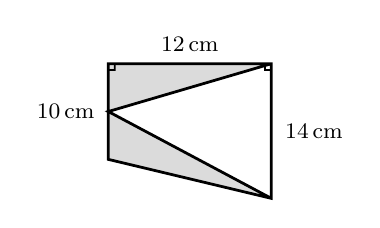
\begin{tikzpicture}[scale=0.45, every node/.style={font=\footnotesize, text=black}]
        \coordinate (T1) at (0,3.8); \coordinate (T2) at (4.6,3.8);
        \coordinate (B2) at (4.6,0); \coordinate (B1) at (0,1.1);
        \coordinate (M1) at (0,2.45);
        \fill[gray!28] (T1)--(T2)--(M1)--cycle;
        \fill[gray!28] (M1)--(B2)--(B1)--cycle;
        \draw[black, line width=1.0pt] (T1)--(T2)--(B2)--(B1)--cycle (T2)--(M1)--(B2);
        \rightbox[0.18cm]{B1}{T1}{T2}\rightbox[0.18cm]{T1}{T2}{B2}
        \node[above=1pt] at (2.3,3.8) {$12\unit{cm}$};
        \node[left=1.5pt] at (0,2.45) {$10\unit{cm}$};
        \node[right=1.5pt] at (4.6,1.9) {$14\unit{cm}$};
      \end{tikzpicture}
    \end{center}
    $S_{\text{ព្នាយ}} = \dfrac{(10+14)\times 12}{2} =$ \blank{1.4cm} $\unit{cm}^2$\\[2.5pt]
    $S_{\text{ត្រីកោណស}} = \dfrac{14 \times 12}{2} =$ \blank{1.4cm} $\unit{cm}^2$\\[2.5pt]
    ដូចនេះ $S_{\text{ប្រផេះ}} =$ \blank{1.4cm} $-$ \blank{1.4cm} $=$ \blank{1.5cm} $\unit{cm}^2$។\\[2.5pt]
    \chkbox\ \textit{បានផ្ទៀងផ្ទាត់ជាមួយដៃគូរួចរាល់}
  \end{tcolorbox}
\end{minipage}\hfill
\begin{minipage}[t]{9.4cm}
  \begin{tcolorbox}[
    enhanced, sharp corners, colback=white, colframe=black,
    boxrule=0.95pt, boxsep=2pt, top=4pt, bottom=4pt, left=5pt, right=5pt, equal height group=e5area4
  ]
    \textbf{ខ. លំហាត់ទី ៦ រូបទី៤ (ទំ.១៩៥)៖} អដ្ឋកោណក្នុងការេ $9\times 9$ កាត់កែង $3\times 3$ បួនជ្រុង៖
    \begin{center}
      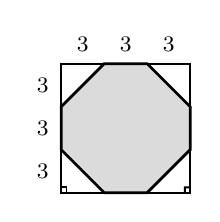
\begin{tikzpicture}[scale=0.42, every node/.style={font=\footnotesize, text=black}]
        \fill[gray!28] (1.3,0)--(2.6,0)--(3.9,1.3)--(3.9,2.6)--(2.6,3.9)--(1.3,3.9)--(0,2.6)--(0,1.3)--cycle;
        \draw[black, line width=0.85pt] (0,0) rectangle (3.9,3.9);
        \draw[black, line width=1.0pt] (1.3,0)--(2.6,0)--(3.9,1.3)--(3.9,2.6)--(2.6,3.9)--(1.3,3.9)--(0,2.6)--(0,1.3)--cycle;
        \rightbox[0.16cm]{0,1.3}{0,0}{1.3,0}\rightbox[0.16cm]{2.6,0}{3.9,0}{3.9,1.3}
        \node[above=1pt] at (0.65,3.9) {$3$}; \node[above=1pt] at (1.95,3.9) {$3$}; \node[above=1pt] at (3.25,3.9) {$3$};
        \node[left=1pt] at (0,3.25) {$3$}; \node[left=1pt] at (0,1.95) {$3$}; \node[left=1pt] at (0,0.65) {$3$};
      \end{tikzpicture}
    \end{center}
    $S = 9^2 - 4\times\left(\frac{1}{2}\times 3\times 3\right) = 81 -$ \blank{1.1cm} $=$ \blank{1.3cm} $\unit{cm}^2$។\\[3.5pt]
    \textbf{គ. បិទបេសកកម្ម E1 (លំហាត់ទី១០ ទំ.១៩៦)៖}\\
    $S = \dfrac{(400+150)\times 500}{2} =$ \blank{2.2cm} $\unit{m}^2 \Rightarrow$ \blank{2.0cm} ផ្ទាំង។\\[3.5pt]
    \textbf{Exit Check៖} ការេ $10\times 10$ កាត់កែង $2\times 2$ ចំនួន ៤ ជ្រុង៖\\
    \chkbox\ \textbf{A.} $96$ \hspace{0.4cm} \chkbox\ \textbf{B.} $92$ \hspace{0.4cm} \chkbox\ \textbf{C.} $84$ \hspace{0.4cm} \chkbox\ \textbf{D.} $98$
  \end{tcolorbox}
\end{minipage}

% ==================== កិច្ចការផ្ទះ (ជំហានទី ៥) ====================
\vspace{4pt}
\begin{tcolorbox}[
  enhanced, sharp corners, colback=panelgray, colframe=black,
  boxrule=1.0pt, boxsep=2pt, top=3.5pt, bottom=3.5pt, left=6pt, right=6pt
]
  {\muol\fontsize{9.0pt}{13pt}\selectfont កិច្ចការផ្ទះបញ្ចប់មេរៀនទី១៤ (សៀវភៅគោល ទំ.១៩៥\enbf{--}១៩៦ — ត្រៀមដែកឈានសម្រាប់មេរៀនទី១៥ ៖ រង្វង់)}\\[2pt]
  $\bullet$ \textbf{លំហាត់ទី ៦ (រូបទី២ និងរូបទី៥ ទំ.១៩៥)៖} គណនាផ្ទៃប្រផេះរូបអក្សរ \en{L} កាត់ត្រីកោណកែង ($14\times 26$) និងអដ្ឋកោណក្នុងចតុកោណកែង $42\times 21$ (មាត់កាត់ $6\times 6$ បួនជ្រុង)។\\
  $\bullet$ \textbf{លំហាត់ទី ៧ (ទំ.១៩៦)៖} គណនាបរិមាត្ររូបមុខផ្ទះខាងលើ និងផ្ទៃក្រឡាព្រមទាំងបរិមាត្រចតុកោណព្នាយ ($b'=15, b=30, h=15$)។
\end{tcolorbox}

\end{document}
